\documentclass[tikz,border=5pt]{standalone}
\usepackage{fontspec}
\setmainfont{Times New Roman}
\usepackage{unicode-math}
\setmathfont{Cambria Math}
\usetikzlibrary{shapes.geometric,positioning,fit,backgrounds,arrows.meta,calc}

\begin{document}
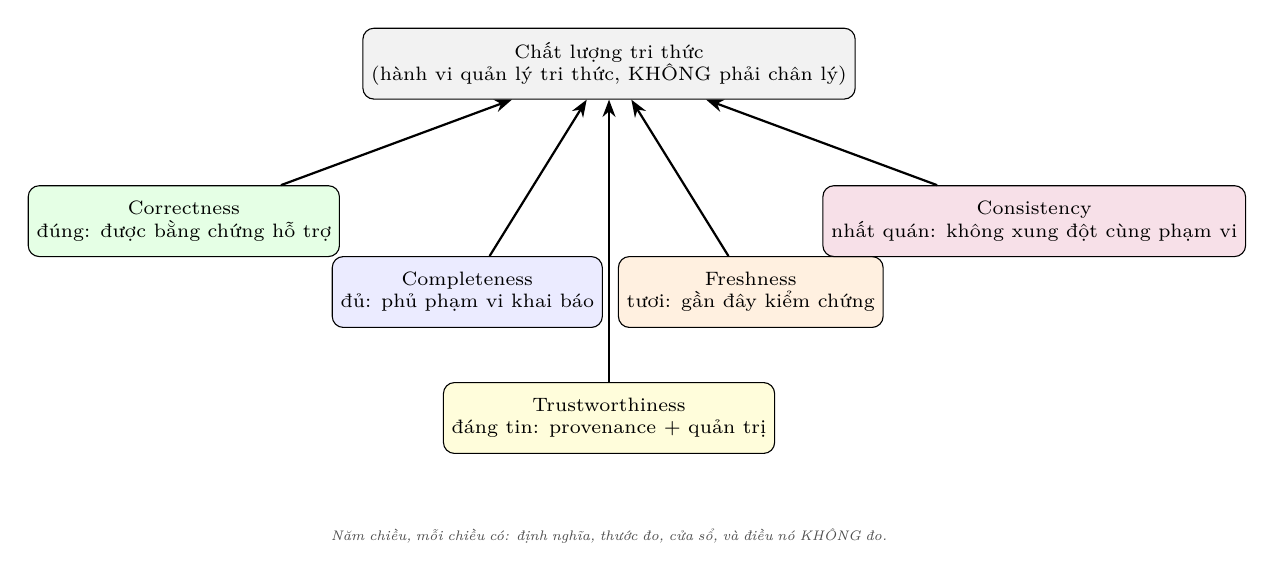
\begin{tikzpicture}[
  box/.style={rectangle, draw, rounded corners, align=center, font=\scriptsize, inner sep=3pt},
  arrow/.style={-{Stealth[length=2.2mm]}, thick},
  label/.style={font=\tiny\itshape, text=gray!60!black},
]

% === FIVE QUALITY DIMENSIONS ===
\node[box, fill=gray!10, minimum width=4.6cm, minimum height=0.9cm] (hub) at (0, 2.9) {Chất lượng tri thức\\
(hành vi quản lý tri thức, KHÔNG phải chân lý)};

\node[box, fill=green!10, minimum width=3.2cm, minimum height=0.9cm] (d1) at (-5.4, 0.9) {Correctness\\đúng: được bằng chứng hỗ trợ};
\node[box, fill=blue!8, minimum width=3.2cm, minimum height=0.9cm] (d2) at (-1.8, 0.0) {Completeness\\đủ: phủ phạm vi khai báo};
\node[box, fill=orange!12, minimum width=3.2cm, minimum height=0.9cm] (d3) at (1.8, 0.0) {Freshness\\tươi: gần đây kiểm chứng};
\node[box, fill=purple!12, minimum width=3.2cm, minimum height=0.9cm] (d4) at (5.4, 0.9) {Consistency\\nhất quán: không xung đột cùng phạm vi};
\node[box, fill=yellow!14, minimum width=3.6cm, minimum height=0.9cm] (d5) at (0, -1.6) {Trustworthiness\\đáng tin: provenance + quản trị};

\draw[arrow] (d1) -- (hub);
\draw[arrow] (d2) -- (hub);
\draw[arrow] (d3) -- (hub);
\draw[arrow] (d4) -- (hub);
\draw[arrow] (d5) -- (hub);

\node[label, align=center, text width=11cm] at (0, -3.1)
  {Năm chiều, mỗi chiều có: định nghĩa, thước đo, cửa sổ, và điều nó KHÔNG đo.};
\end{tikzpicture}
\end{document}